\documentclass[%
%   preprint,
superscriptaddress,
%groupedaddress,
%unsortedaddress,
%runinaddress,
%frontmatterverbose,
%preprint,
%showpacs,preprintnumbers,
%nofootinbib,
%nobibnotes,
%bibnotes,
%twocolumn,
amsmath,amssymb,
aps,
pre,
%prb,
%rmp,
%prstab,
%prstper,
floatfix,
]{revtex4-2}

\usepackage{graphicx}% Include figure files
\usepackage{dcolumn}% Align table columns on decimal point
\usepackage{bm}% bold math
\usepackage{hyperref}% add hypertext capabilities
\usepackage{color}
\usepackage{verbatim}
\graphicspath{{./fig/}}
%\usepackage{epstopdf}
%\usepackage{auto-pst-pdf}

%todo Chris: Write about 1/1 mode
%todo Chris: Write results/figure explanation section

%todo Ralf: Write q_\infty derivation
%todo Ralf: Read and improve introduction. 


\begin{document}
\title{Toy model for the sawtooth oscillation}
\author{Ralf Mackenbach}
\affiliation{Princeton Plasma Physics Laboratory, Princeton University, Princeton, New Jersey, USA}
\author{C. B. Smiet}
\affiliation{Princeton Plasma Physics Laboratory, Princeton University, Princeton, New Jersey, USA}
\affiliation{Huygens-Kamerlingh Onnes Laboratory, Leiden University, P.O.\ Box 9504, 2300 RA Leiden, The Netherlands}

\begin{abstract}
  The Sawtooth crash is an instability occurring in the core of a tokamak plasma that redistributes the temperature and pressure in the core region.
  In the Kadomtsev model the crash is caused by a 1/1 internal kink that reconnects the hot plasma within the core region.
  In this paper we present a minimal analytical model with two free parameters that reproduces the predicted changes in topology.
  This paints an intuitive picture of how the magnetic topology changes during a sawtooth crash.
\end{abstract}
\maketitle

The sawtooth crash has been observed in tokamak fusion reactors since 1974 \cite{von1974studies, vershkov1974role}.
Because of the temperature dependent Spitzer resistivity, the plasma current that creates the rotational transform in the reactor preferentially concentrates on the hottest plasma region near the magnetic axis.
This decreases the safety factor (increases the field line winding) around the core.
Current diffuses onto the core of the tokamak on a slow, resistive timescale, until a fast instability is triggered at a specific value of $q_0$ (the safety factor on the magnetic axis)
At a specific value of $q_0$ a fast instability is triggered that redistributes the plasma in the core region, and leads to a flat temperature and pressure profile.
This instability redistributes the poloidal and toroidal flux, resulting in a higher $q_0$.
The sawtooth cycle resets, and current slowly accumulates on the axis until the instability is triggered again.

A full numerical simulation of a sawtoothing discharge is shown in figure [REF]. [ADD ANIMATED GIF TO PAPER]

One of the most enduring models for the sawtooth was presented by Kadomtsev~\cite{kadomtsev1975disruptive}.
In this model the region within the $q=1$ surface becomes susceptible to an internal kink mode, a resistive tearing instability of the $q=1$ surface, or both~\cite{coppi1976resistive}.
The plasma in the core reconnects with cold plasma from outside the $q=1$ surface along a helical ribbon on the $q=1$ surface, and is deposited in a growing 1/1 island.
This growing island eventually completely displaces the hot core, and the temperature and current are re-distributed.
After the crash, the hot core is completely replaced by the $1/1$ island, which has $q_0=1$.

In this paper we present a simple analytical toy model for the above process that uses two independent parameters to reproduce the predicted change in topology: a 1/1 internal kink that displaces the core, and a linear interpolation between the initial and final flux predicted by kadomtsev.
Other expressions for the time-dependent magnetic topology during the sawtooth crash have been presented by Kolesnichenko~\cite{kolesnichenko1996theory} and Jaulmes~\cite{jaulmes2014redistribution}.
These works calculate the intermediate states in the Kadomtsev reconnection process, whereas the current treatment separates the reconnection phase into two separate and independent perturbations, resulting in a more analytically tractable and intuitive picture, at the cost of accuracy.

\section*{Initial magnetic field}
The magnetic field in a tokamak ideally consists of nested toroidal magnetic surfaces with a monotonically increasing $q$-profile.
We generate such an equilibrium field using a poloidal flux function $\psi_p(R, Z)$ and a toroidal current function $I(\psi_p)$.
The coordinates used are illustrated in figure~\ref{fig:coords}.
Physically $\psi_p$ represents the amount of flux through the circular disc with radius R centered on the $Z$ axis (indicated by the green circle in figure~\ref{fig:coords}.
$I$, which is sometimes called $F$ or $G$, represents the current through the same surface divided by 2$\pi$.
\begin{figure}\label{fig:coords}
  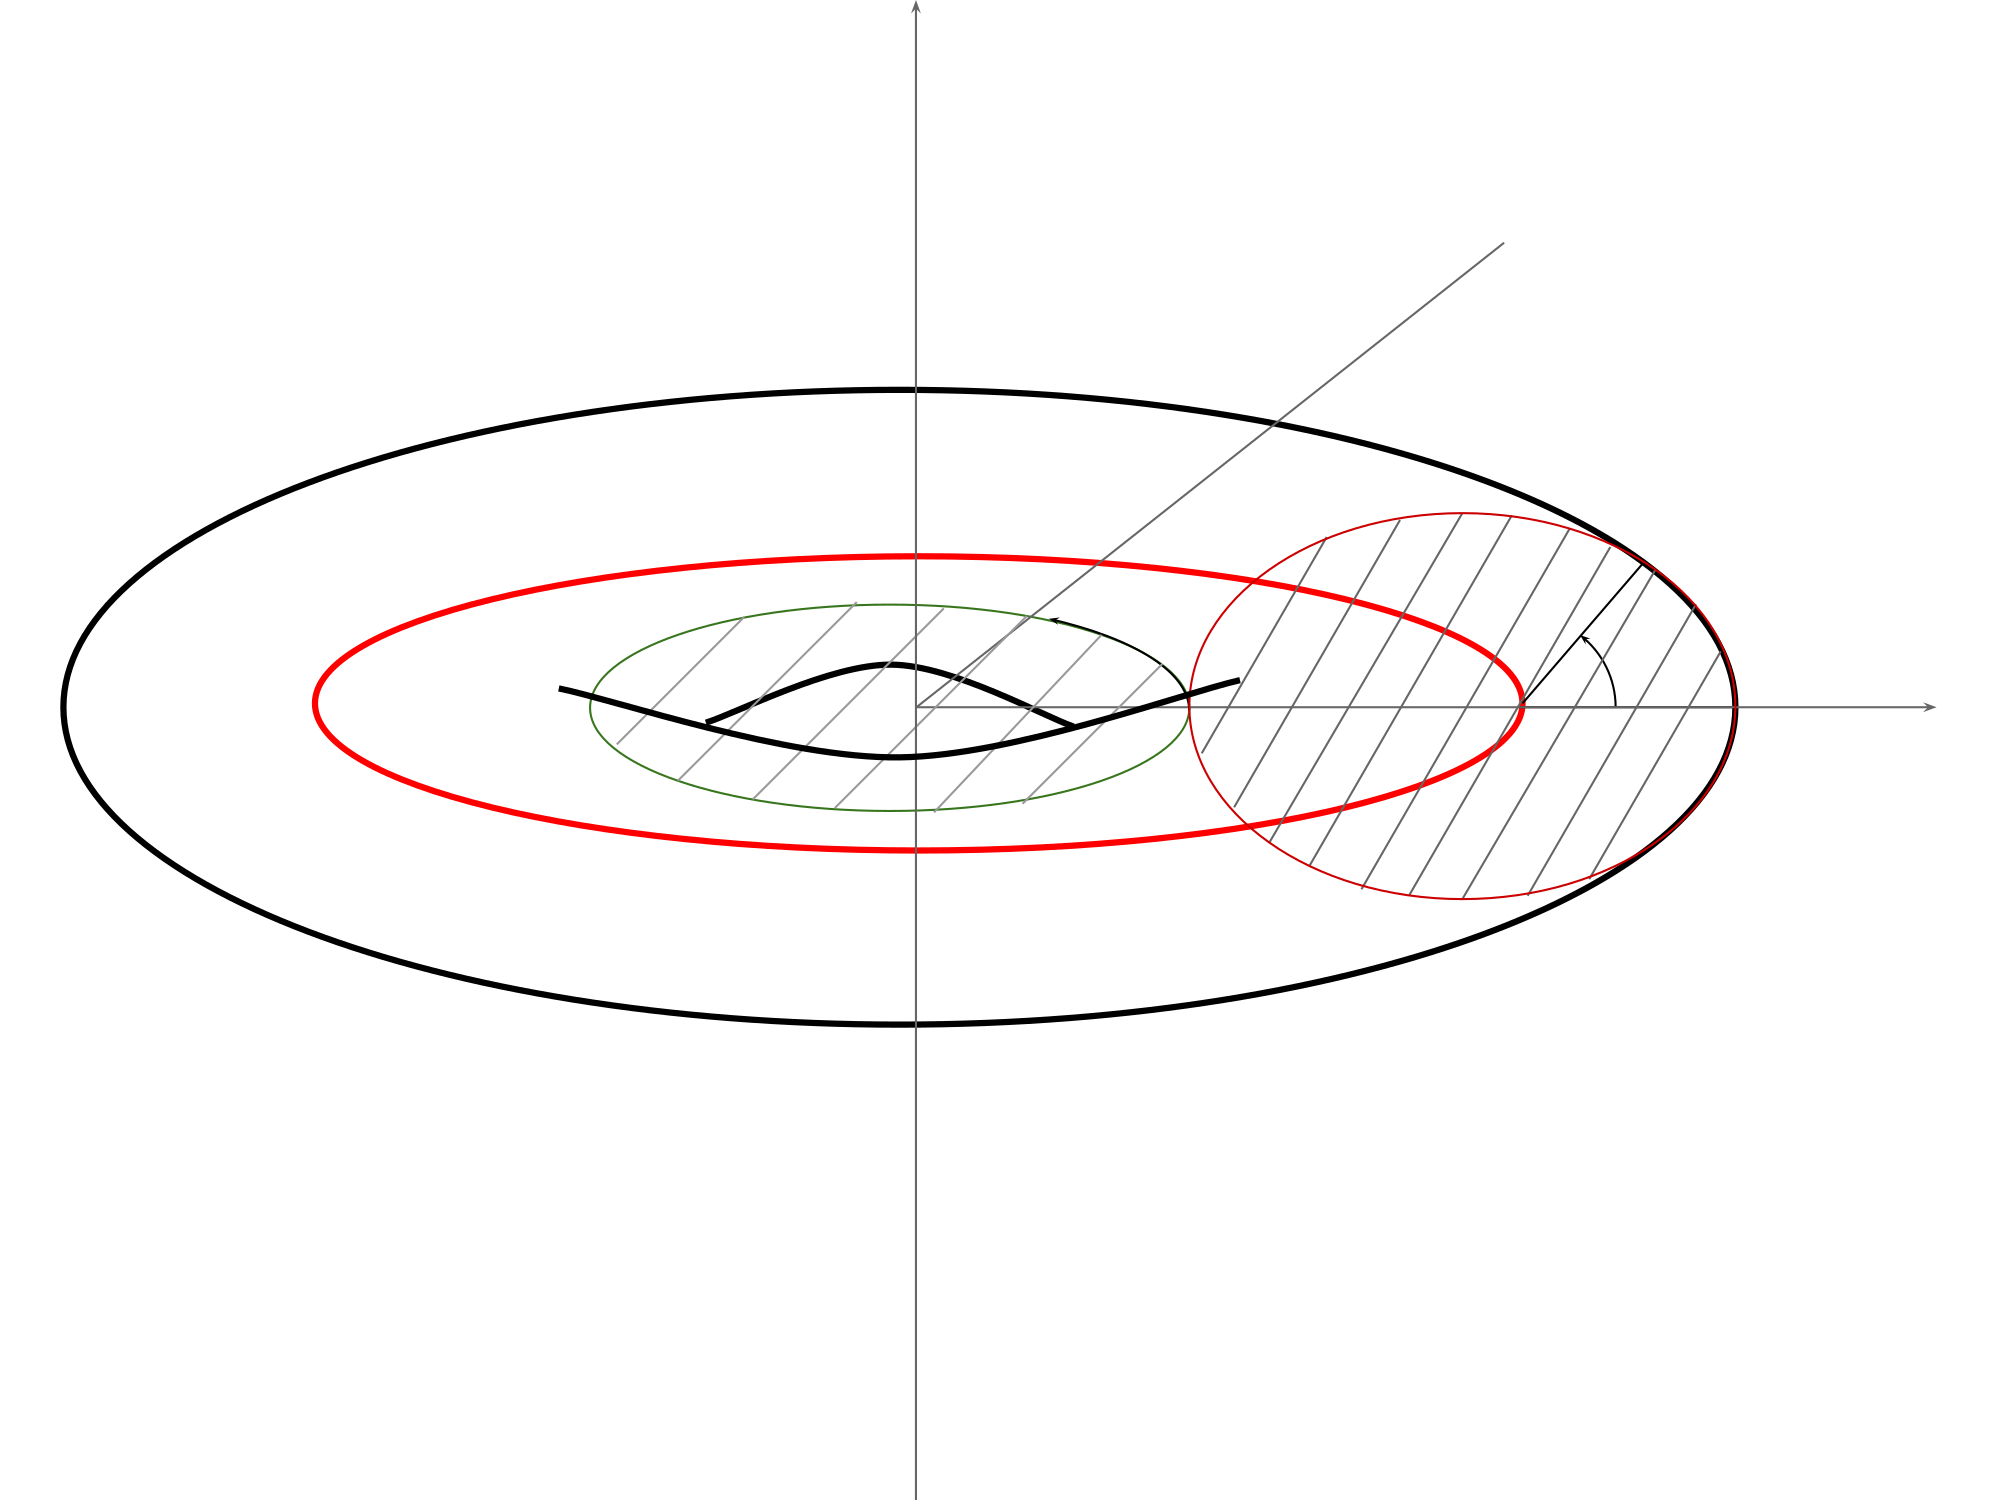
\includegraphics[width=0.7\textwidth]{fig/torus.png}
  \caption{Coordinates used for generating the magnetic field. }
\end{figure}

The magnetic fields are calculated from $\psi_p$ and $I$ using:
\begin{equation}\label{eq:unperturbed}
  B_R = -\frac{1}{R} \frac{\partial \psi_p}{\partial z}, \quad B_z= \frac{1}{R} \frac{\partial
  \psi_p}{\partial R}, \quad
  B_\phi = \frac{1}{R} I.
\end{equation}

For the poloidal flux function we use
\begin{equation}
  \psi_p = a^2
\end{equation}
where $a=\sqrt{Z^2 + (R-R_0)^2}$ with $R_0$ the location of the magnetic axis.
The surfaces of constant $\psi_p$, which are magnetic surfaces, are thus circular-cross-section concentric tori around a magnetic axis located at $R=R_0$.

For our current function $I$ we choose the following relation:
\begin{equation}
  I(\psi) = 2(q_0 + \gamma \psi_p)\sqrt{R_0-\psi_p}
\end{equation}


The safety factor on each surface is calculated through~\cite{wesson2011tokamaks}:
\begin{equation}\label{eq:qprofint}
  q=\frac{1}{2\pi} \oint \frac{1}{R}\frac{B_\theta}{B_p}\mathrm{d} l,
\end{equation}
where $B_p=\sqrt{B_R^2+B_Z^2}$ is the magnitude of the poloidal magnetic field.
The integration is carried out over a magnetic surface, which in the circular-cross-section concentric toroidal geometry can be done analytically.
The quantity $R B_p$ is constant in this geometry, so we get:
\begin{equation}
  q = \frac{1}{2\pi} \frac{I(\psi_p)}{RB_p}\oint \frac{1}{R} \mathrm{d}l.
\end{equation}
We evaluate the integral by integrating over $\theta$ and using the identities $R=R_0 +a \cos(\theta)$ and $\mathrm{d}l = a \mathrm{d}\theta$ to yield:
\begin{equation}
  \oint \frac{1}{R} \mathrm{d}l = \int_0^{2\pi} \frac{a}{R_0 + a \cos(\theta)} \mathrm{d}l =
  \frac{2\pi a}{\sqrt{R_0^2 -a^2}}
\end{equation}
In the above integration we used the facts that $R_0>0$ and $R_0>a>0$.
This explains our choice of the function $I$, whose square root term cancels against the integrand, giving us the safety factor profile of:
\begin{equation}
  q=q_0 + \gamma \psi_p.
\end{equation}

The expressions in \ref{eq:unperturbed} thus give us an axisymmetric magnetic field where field lines lie on nested concentric toroidal magnetic surfaces with monotonically increasing safety factor.
For this calculation we choose the parameters $\gamma=1$ and $q_0=2/3$, thus yielding a
This field has no shafranov shift (a shift of the magnetic axis outwards, induced by plasma pressure).
Including a shafranov shift would make the factor $RB_p$ non-constant on a magnetic surface, thus requiring numerical integration for the evaluation of the integral in~\ref{eq:qprofint}.

\section*{Internal Kink}
We add a

\begin{equation}\label{eq:kinky}
{\rm[PLACEHOLDER]}
\end{equation}

\section*{The Kadomtsev final state}

\section{Perturbing the magnetic field}


We construct a Poincar\'e plot of the magnetic field. 
A Poincar\'e plot gives a good sense of the magnetic connectivity. 
It is calculated by taking a point in the $\phi=0$ plane, numerically calculating the magnetic field line passing through that point, and noting the location where the that field line passes through the plane every time it does so. 
If a field line fills out a magnetic surface, and the the field line is followed for long enough, then the Poincar\'e section will start to fill out the circle that corresponds with the intersection of that magnetic surface and the $\phi=0$ plane. 
This procedure is done for 100 different field lines, and each field line is given a different color.
The Poincar\'e section for the unperturbed field (equation~\eqref{eq:unperturbed}) is visible in figure [REF TO FIG]. 

We also calculate the safety factor of each field line, buy counting the number of times it winds around the magnetic axis of the unperturbed field. 
This information is shown below the Poincar\'e plot. 

We can now perturb the initial magnetic field $B_0$ with the two perturbations $B_{1,1}$ and $B_\infty -B_0$ in the following way: 
\begin{equation}\label{eq:totalfield}
    \delta B =  B_0 + \alpha B_{1,1}+ \epsilon (B_\infty -B_0). 
\end{equation}
The factor $\alpha$ now determines the strength of the internal kink perturbation, whereas $\epsilon$ linearly interpolates between the initial state and the final state predicted by the Kadomtsev model. 

The effects of these two perturbations on the field can be interactively explored in figure [REF]. 
In figure [REF] different combinations of $\alpha$ and $\epsilon$ can be specifed along a path, and a Poincar\e plot of every set of ($\alpha$, $\epsilon$) along this path will be computed. 

When a path is chosen such that only $\alpha$ varies, but $\epsilon$ remains zero, we see the effect of the internal kink on the magnetic configuration. 
As can be seen, this results in a shifting of the magnetic axis in the direction of the perturbation, and back again. 

When only $\epsilon$ is varied, but $alpha$ is kept constant, the magnetic structure does not change at all. 
The only change is seen in the plot of the safety factor, which just linearly interpolates between the initial value of $q_0=2/3$ [change!] and $q_0=1$ in the final Kadomtsev state. 

An interesting thing happens when we first apply the internal kink $alpha$, and with this perturbation in place, start increasing $\epsilon$. 
As soon as $\epsilon$ is non-zero, we see a drastic change in the magnetic structure. 
We see a set of crescent-moon shaped curves in the Poincar\'e plot. 
These are caused by field lines lying on a new type of magnetic surface, that does not surround the magnetic axis anymore. 
Such a structure is called a \emph{magnetic island}. 
Because this structure has appeared on the surface where previously $q=n/m=1/1$, this is called a $1/1$-island. 
Opposite to the center of the island, we see the point where the tips of the crescent moon touch. 
The point where the tips touch exaclty is called an X-point. 
There is a field line at the center of the 'X' that comes back to itself after one rotation. 

As we continue to increase  $\epsilon$, the size of the island keeps increasing, even when we keep $\alpha$ constant. 
What $\epsilon$ does is to flatten the safety factor profile, bringing $q$ closer to 1 everywhere in the core region.
As $q$ gets closer to 1, it means that field lines rotate around exactly once poloidally per toroidal rotation. 
The perturbation $B_{1,1}$ given by equation~\eqref{eq:kinky} has exactly the same angular dependence. 
That means that the effect of $B_{1,1}$ on the trajectory of a field line gets larger and larger, the closer $q$ gets to 1. 
If $B_{1,1}$ adds a little push to the direction of a field line inone location, it will be adding the same push further along, and at every point, eventually completely changing the trajectory of the field line. 
This effect, where the magnetic structure is strongly affected even by a very small perturabtion, if the effect accumulates in this way, is called \emph{magnetic resonance} or just resonance. 

As we change $\epsilon$ towards 1, the safety factor becomes flatter, and closer to 1. 
This means that the effect of the internal kink becomes stronger, pushing the original magnetic axis further out, and at the same time increasing the size of the island.
When $\epsilon$ gets really close to 1, the original axis gets closer and closer to the X-point, and fewer and field lines surround it, while more and more field lines are part of the island. 
Before $\epsilon$ reaches 1, the effect of the kink is already so strong, that the original axis is pushed into the X-point, and both dissappear!

The island has grown so large that it has completely taken over, and the original axis has completely dissappeared. 
If we have not returned $\alpha$ to zero, the magnetic field in the core will still be strongly distorted. 
But the drive for such a perturbation has dissappeared now that the safety factor is above 1 everythwere, so the last step should be to return $\alpha$ to 1, and see that the magnetic structure becomes axisymmetric again. 
The final step is to return to the original profile with $q_0<1$, from which the cycle starts anew. 

- fast and slow
- kink triggering
- realistic path

\section*{Conclusions and Discussion}
The model we have presented above gives a very simple intuitive picture of the minimal perturbations that result in the Kadomtsev sawtooth. 
We take two effects; the ideal kink and a linerar interpolation between two axisymmetric states, to reproduce the changes in magnetic topology that constitute the Kadomtsev satwooth. 
A minimal model needs at least two parameters. Whether these two are simplest seems reasonable. 

The evolution of the magnetic structure exhibited by our model is probably simpler than what would be physically realized. 
A better approximation would be given by the models presented in~\cite{kolesnichenko1996theory, jaulmes2014redistribution}, as these models give a physical picture for the intermediate states between initial and final state. 
Nevertheless, the states in these models will also not correspond exactly to the actual magnetic state during the sawtooth crash, as there will be many other effects present such as current sheet formation, deformation of the shape of the original axis, etc.


\bibliographystyle{naturemag}
\bibliography{refs}

\end{document}
